%----------------------------------------------------------------------------------------
%	PACKAGES AND OTHER DOCUMENT CONFIGURATIONS
%----------------------------------------------------------------------------------------

\documentclass[twoside]{article}

\usepackage[sc]{mathpazo} % Use the Palatino font
\usepackage[T1]{fontenc} % Use 8-bit encoding that has 256 glyphs
\linespread{1.05} % Line spacing - Palatino needs more space between lines
\usepackage{microtype} % Slightly tweak font spacing for aesthetics

\usepackage[english]{babel} % Language hyphenation and typographical rules

\usepackage[hmarginratio=1:1,top=32mm,columnsep=20pt]{geometry} % Document margins
\usepackage[hang, small,labelfont=bf,up,textfont=it,up]{caption} % Custom captions under/above floats in tables or figures
\usepackage{booktabs} % Horizontal rules in tables

\usepackage{lettrine} % The lettrine is the first enlarged letter at the beginning of the text

\usepackage{enumitem} % Customized lists
\setlist[itemize]{noitemsep} % Make itemize lists more compact

\usepackage{titlesec} % Allows customization of titles
\renewcommand\thesection{\Roman{section}} % Roman numerals for the sections
\renewcommand\thesubsection{\roman{subsection}} % roman numerals for subsections
\titleformat{\section}[block]{\large\scshape\centering}{\thesection.}{1em}{} % Change the look of the section titles
\titleformat{\subsection}[block]{\large}{\thesubsection.}{1em}{} % Change the look of the section titles

\usepackage{fancyhdr} % Headers and footers
\pagestyle{fancy} % All pages have headers and footers
\fancyhead{} % Blank out the default header
\fancyfoot{} % Blank out the default footer
\fancyhead[C]{TensorFlow Speech Recognition $\bullet$ May 2018} % Custom header text
\fancyfoot[RO,LE]{\thepage} % Custom footer text

\usepackage{titling} % Customizing the title section

\usepackage{hyperref} % For hyperlinks in the PDF

\usepackage{multicol}
\usepackage{graphicx}
\graphicspath{{img/}}
\usepackage{float}
\renewcommand{\figurename}{Fig.}

\usepackage{amssymb,amsmath,amsthm}
\newtheorem{theorem}{Theorem}
\newtheorem{defn}{Definition}

\newcommand{\code}[1]{\texttt{#1}}

\newenvironment{Figure}
  {\par\medskip\noindent\minipage{\linewidth}}
  {\endminipage\par\medskip}

%----------------------------------------------------------------------------------------
%	TITLE SECTION
%----------------------------------------------------------------------------------------

\setlength{\droptitle}{-4\baselineskip} % Move the title up

\pretitle{\begin{center}\Huge\bfseries} % Article title formatting
\posttitle{\end{center}} % Article title closing formatting
\title{TensorFlow Speech Recognition} % Article title

\author{%
\textsc{Petra Br\v{c}i\'c}\\% \\[1ex] 
\normalsize Applied Mathematics \\
\normalsize \href{mailto:petrabrcic94@gmail.com}{petrabrcic94@gmail.com} 
\and
\textsc{Ivan \v{C}eh}\\% \\[1ex] 
\normalsize Computer Science \\
\normalsize \href{mailto:ivan.ceh1234@gmail.com}{ivan.ceh1234@gmail.com} 
\and
\textsc{Sandro Lovni\v{c}ki}\\% \\[1ex] 
\normalsize Computer Science \\ 
\normalsize \href{mailto:lovnicki.sandro@gmail.com}{lovnicki.sandro@gmail.com}
}

\date{\today} 
\renewcommand{\maketitlehookd}{%
\noindent \textbf{\\Abstract:} We are witnessing the significant development of the blooming relationship between science and technology. Humanity is striving on making everyday life easier and more controllable by the integration of the intelligent machines. We want to control those machine easier, such as by spoken commands. This is where this project comes in and answers that question.
\\\\
\textbf{Keywords:} tensorflow, speech recognition, audio recognition, feature extraction, MFCC, convolutional neural network.
}


%----------------------------------------------------------------------------------------

\begin{document}

% Print the title and table of contents
\maketitle
%\tableofcontents
%\newpage

%----------------------------------------------------------------------------------------
%	ARTICLE CONTENTS
%----------------------------------------------------------------------------------------
\begin{multicols}{2}

\section{Introduction}
This project was given by Kaggle as Tensorflow challenge\footnote{https://www.kaggle.com/c/tensorflow-speech-recognition-challenge}, where the task is to correctly classify the audio recording of a spoken words. In this paper, we discuss audio transformations needed to extract shared features to feed the convolutional neural network classifier and present results we obtained on couple of examples. All of the code as well as usage instructions can be found at our \hyperref[https://github.com/Qkvad/SpeechRecognition]{GitHub repository}\footnote{https://github.com/Qkvad/SpeechRecognition}.

%------------------------------------------------
\section{Data}
Dataset was given by Tensorflow as one second audio clips of different words spoken by different people. Dataset can automaticly be downloaded when starting the train part of machine learning solution to the problem. 
The goal is to have a model that tries to classify a one second audio clip as either silence, an unknown word, "yes", "no", "up", "down", "left", "right", "on", "off", "stop" and "go", even though more words can be found in the dataset and included in the training process. Each of the words is separated into files named as the recordings of the word they present. In order to make these clips as realistic as they would be in real life, the background noise is added in preprocess part of the code. There is a file of few background noises within the dataset that is downloaded. 
Each audio file is encoded with the id of the person who recorded the word, followed by nohash and a number from 0, specifing the time the same person recorded the word.  
Apart from the audio files that take up the majority of the data file, testing and validation lists can be found too. Each of those text file contains a list of the audio clips so that dataset can be patitioned in training, validation and test set. 
\subsection{Preprocessing}
In order to feed our neural network with the data, we first need to process it. Neural network is fed by the image, so we need to tranform the audio file to a spectrogram. Spectrogram is a visual representation of the spectrum of frequencies of sound or other signal as they vary in time. Spectrograms can be generated by an optical spectrometer, a bank of band-pass filters or by Fourier transorm. 
First, let us observe what the data looks like after reading the audio file. \\
 
\begin{Figure}
	\centering
	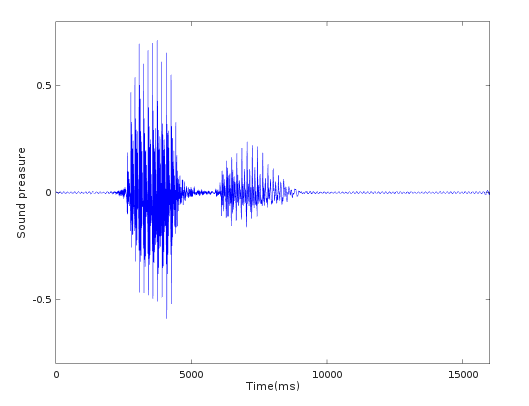
\includegraphics[width=1.0\textwidth]{happy-read1}
	\captionof{figure}{Waveform for audio 'happy'}
	\label{img:pocetnoStanje}
\end{Figure}

Creating a spectrogram using FFT is a digital process. Digitally sampled data (which ours is), in time domain, is broken up into chunks, which usually overlap, and Fourier transformed to calculate the magnitude of the frequency spectrum for each chunk. Each chunk then corresponds to a vertical line in the image; a measurement of magnitude versus frequency for a specific moment in time (the midpoint of the chunk). These spectrums or time plots are then laid side by side to form the image or a three-dimensional surface, or slightly overlapped in various ways, i.e. windowing. This process essentially corresponds to computing the squared magnitude of the short-time Fourier transform (STFT) of the signal x(t) - that is, for a window $\omega$,
\[ spectrogram(t,\omega)=|STFT(t,\omega)|^2 ,\]
where 
\begin{align*} STFT \lbrace x[n] \rbrace (m,\omega)&\equiv X(m,\omega) \\ 
&=\sum_{n=-\infty}^{\infty} x[n]\omega [n-m]e^{-j\omega n}.
\end{align*}
The STFT is performed on a computer so it uses the FFT (Fast Fourier Transform), so all the variables are discrete and quantized. \\
After running our code in Octave to generate spectrogram yield the figure~\ref{img:specgramStanje} \\
\begin{Figure}
	\centering
	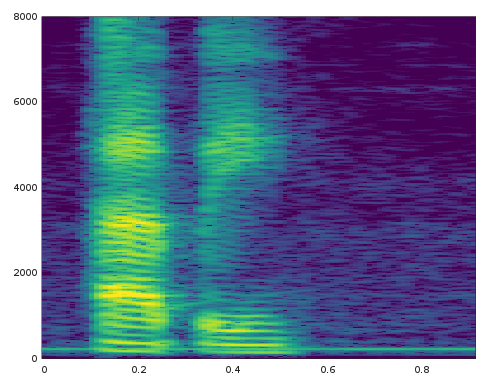
\includegraphics[width=1.0\textwidth]{happy-specgram}
	\captionof{figure}{Spectogram for audio 'happy'}
	\label{img:specgramStanje}
\end{Figure}
Our code works slightly different, first we scale the volume, then we shift it in time, add background noise and then calculate spectrogram. But for all the features of spectrogram to be easily visible on the paper form, we added the octave function to obtain the standard version of the spectrogram.\\
There is one more thing we have to dig into, that is getting from spectrogram to the image that is going to feed the machine learning algorithm. Final output of the preprocess is mel-frequency cepstrum \footnote{Cepstrum (the name derived by reversing the first four letters of "spectrum", whereas operations on cepstra are labeled quefrency analysis, liftering or cepstral analysis) is the result of IFT of the logarithm of the estimated spectrum of a signal} coefficients (MFCCs), the coefficients that make up an MFC. MFC is a representation of the short-term power spectrum of a sound, based on a linear cosine transform of a log power spectrum on a nonlinear mel scale of frequency. This frequency wraping can allow for better representation of sound in audio compression. \\
MFCCs are derived as follows:
\begin{enumerate}
	\item Take the Fourier transform of (a window excerpt of) a signal
	\item Map the powers of the spectrum obtained above onto the mel scale, using triangular overlapping windows
	\item Take the logs of the powers at each of the mel frequencies
	\item Take the discrete cosine transform of the list of mel log powers, as if it were a signal
	\item The MFCCs are the amplitued of the resulting spectrum.
\end{enumerate}
%------------------------------------------------
\section{Machine Learning}
In order to classify processed audio data into known classes ("up","down",\ldots), we use a neural network model, specifically - a convolutional neural network (CNN). It is important to notice that audio samples corresponding to the same word need not to "look" the same. For example, one speaker may had began speaking later than the other. CNNs have had the most success in dealing with classifying such data and we say that CNN model is thus \emph{spatially invariant}.

Specifically, as is reported in~\cite{our-conv}, CNNs outperform Deep Neural Networks which outperform Hidden Markov Model system, which is a commonly used technique for keyword spotting.\\
To put it simply and stress this fact's importance, we can write
\[ CNN > DNN > HMM \]
where $> = \{(x,y): x,y \text{ are classifiers}\}$ and $(x,y) \in >$ if and only if $x$ performs better that $y$ on a given dataset.

\subsection{Convolutional Neural Network}
We use a convolutional neural network model described in~\cite{our-conv}, with two layers or convolution. The task of convolution layers is to extract features in a spatially invariant manner and it is their output that finally goes into fully connected hidden layers such as in ordinary neural network.

\subsection{Training}
To be honest, training a convolutional neural network with our dataset of over $100000$ audio samples was not a walk in the park. On a fairly strong laptop, it took us about 19 hours for $15000$ training steps with learning rate of $0.001$ and $3000$ training steps with learning rate $0.0001$ for finner descent.

Some of the important parameters for training the model are: \code{wanted\_words}, \code{batch\_size}, \code{learning\_rate}, \code{how\_many\_training\_steps}, \code{clip\_duration\_ms}, \code{data\_dir}, \ldots

Most important parameters that control the preprocessing are: \code{background\_volume}, \code{silence\_percentage}, \code{unknown\_percentage}, \code{time\_shift\_ms}, \code{window\_size\_ms},\\ \code{window\_stride\_ms}, \code{dct\_coefficient\_count}, \ldots

Let us observe the confusion matrices and accuracy of our model after $4000$ steps and at the end of training. Classes are listed in order: silence, unknown, yes, no, up, down, left, right, on, off, stop, go.

\begin{Figure}
	\centering
	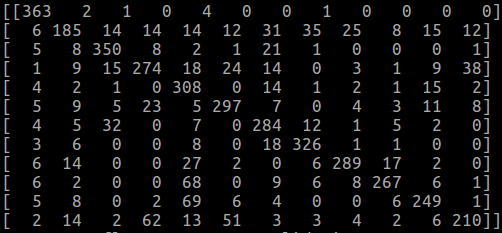
\includegraphics[width=0.8\textwidth]{train_4000}
	\captionof{figure}{Confusion matrix after 4000 train steps}
	\label{img:tr-4000}
\end{Figure}

\begin{Figure}
	\centering
	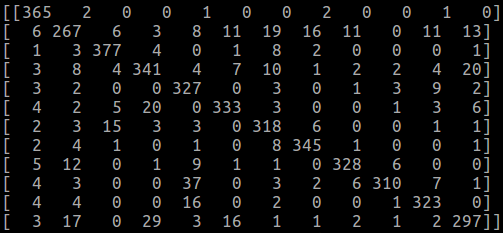
\includegraphics[width=0.8\textwidth]{train_18000}
	\captionof{figure}{Confusion matrix after 18000 train steps}
	\label{img:tr-4000}
\end{Figure}

\noindent We obtained total accuracy of $88,4\%$. As expected, the two classes hardest to distinguish are "no" and "go". 

\subsection{Application}
Now, to see this trained model in action, we give it some easy and also some hard audio files to classify to demonstrate it's power.\\

First, the easy part, let's predict a word "yes" without much background noise. It's read audio file and corresponding MFCC that our model obtains are given in figure~\ref{img:yes-clean}

\begin{Figure}
	\centering
	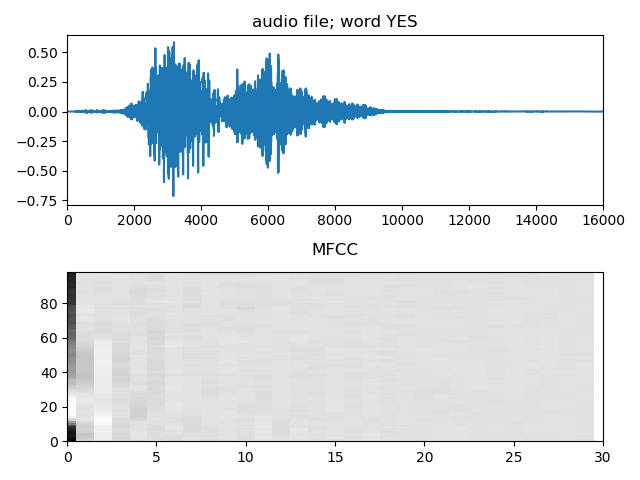
\includegraphics[width=0.8\textwidth]{yes_clean}
	\captionof{figure}{Audio recording of a word "yes"}
	\label{img:yes-clean}
\end{Figure}

The model prediction is as follows:
\begin{itemize}
	\item yes (score = 0.99882)
	\item \_unknown\_ (score = 0.00062)
	\item left (score = 0.00052)
\end{itemize}

Now we feed our model with extremely noised and shifted audio data for "yes". 
\begin{Figure}
	\centering
	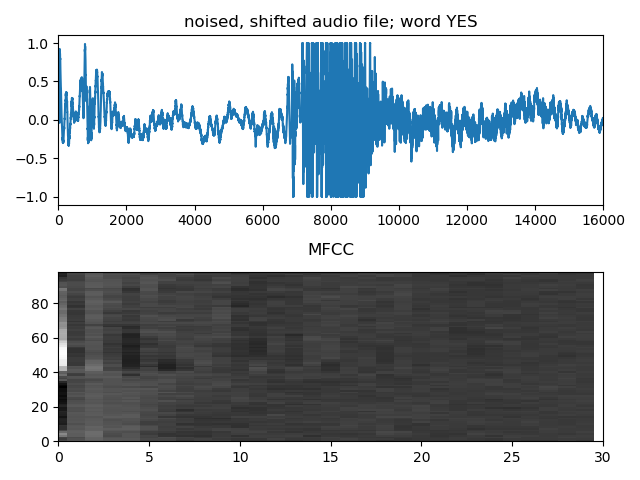
\includegraphics[width=0.8\textwidth]{yes_noised}
	\captionof{figure}{Extreme audio recording of a word "yes"}
	\label{img:yes-noised}
\end{Figure}

Although this is extremely distorted and noised, it seems that our model is pretty confident predicting the following:
\begin{itemize}
	\item yes (score = 0.85262)
	\item left (score = 0.07611)
	\item \_unknown\_ (score = 0.02981)
\end{itemize}




%------------------------------------------------
\section{Different Approaches}


%------------------------------------------------


%----------------------------------------------------------------------------------------
%	REFERENCE LIST
%----------------------------------------------------------------------------------------

\begin{thebibliography}{99}

\bibitem[1]{our-conv}
Tara N. Sainath, Carolina Parada.
\newblock Convolutional Neural Networks for Small-footprint Keyword Spotting

\bibitem[2]{mfcc-feat-ex}
Shikha Gupta, Jafreezal Jaafar, Wan Fatimah wan Ahmad, Arpit Bansal.
\newblock Feature Extraction Using MFCC

\bibitem[3]{methods-1}
Namrata Dave.
\newblock Feature Extraction Methods LPC, PLP and MFCC In Speech Recognition

\bibitem[4]{feat_ex-methods}
Urmila Shrawankar, Vilas Thakare.
\newblock Techniques for Feature Extraction in Speech Recognition System: A Comparative Study

\end{thebibliography}

%----------------------------------------------------------------------------------------

\end{multicols}{2}
\end{document}

